\documentclass[a4paper]{report}
\usepackage{RJournal}
\usepackage[round]{natbib}
\bibliographystyle{abbrvnat}

%% load any required packages here

\begin{document}

%% do not edit, for illustration only
\fancyhf{}
\fancyhead[LO,RE]{\textsc{Contributed Article}}
\fancyhead[RO,LE]{\thepage}
\fancyfoot[L]{The R Journal Vol. X/Y, Month, Year}
\fancyfoot[R]{ISSN 2073-4859}

%% replace RJtemplate with your article
\begin{article}
%%%%%%%%%%%%%%%%%%%%%%%%%%%%%

\title{makeR: An R Package for Managing Document Templates and Versions}
\author{by Jason M. Bryer}

\maketitle

\abstract{
The idea of build automation is not new. \href{http://www.gnu.org/s/make/}{GNU Make} and \href{http://ant.apache.org}{Java Ant} are well established and robust build automation systems but require the use and installation of additional software. The \pkg{makeR} package provides a simplified framework written entirely in R to manage Sweave projects where multiple versions are created based upon a single source repository. For example, a monthly report where each version is identical, with perhaps the exception of easily extracted properties (e.g. date ranges for data extraction, title, etc.). An example project summarizing recent posts from R-Bloggers is provided.
}

R \citep{rcore}, \LaTeX{} \citep{latex}, and Sweave \citep{sweave} have proven to be incredibly useful for conducting reproducible research. However, managing document versions within R is limited. The \pkg{makeR} package attempts to provide the same ease-of-use for document versioning that the \pkg{devtools} \citep{devtools} and \pkg{ProjectTemplate} \citep{projecttemplate} packages have provided for package development and data analysis, respectively. This package attempts to solve the problem where multiple versions of a document are required but the underlying analysis and typesetting code remains static or can be abstracted through the use of variables or properties. For example, many researchers conduct monthly, quarterly, or annual reports where the only difference from version-to-version, from an analysis and typesetting perspective, is the data input. Clearly R and \LaTeX{} are an ideal solution to this problem. The \pkg{makeR} package provides a framework to automate the process of generating new documents from a single source repository.

\begin{figure*}
\vspace*{.1in}
\framebox[\textwidth]{\hfill \raisebox{0in}{\rule{0in}{0in}}
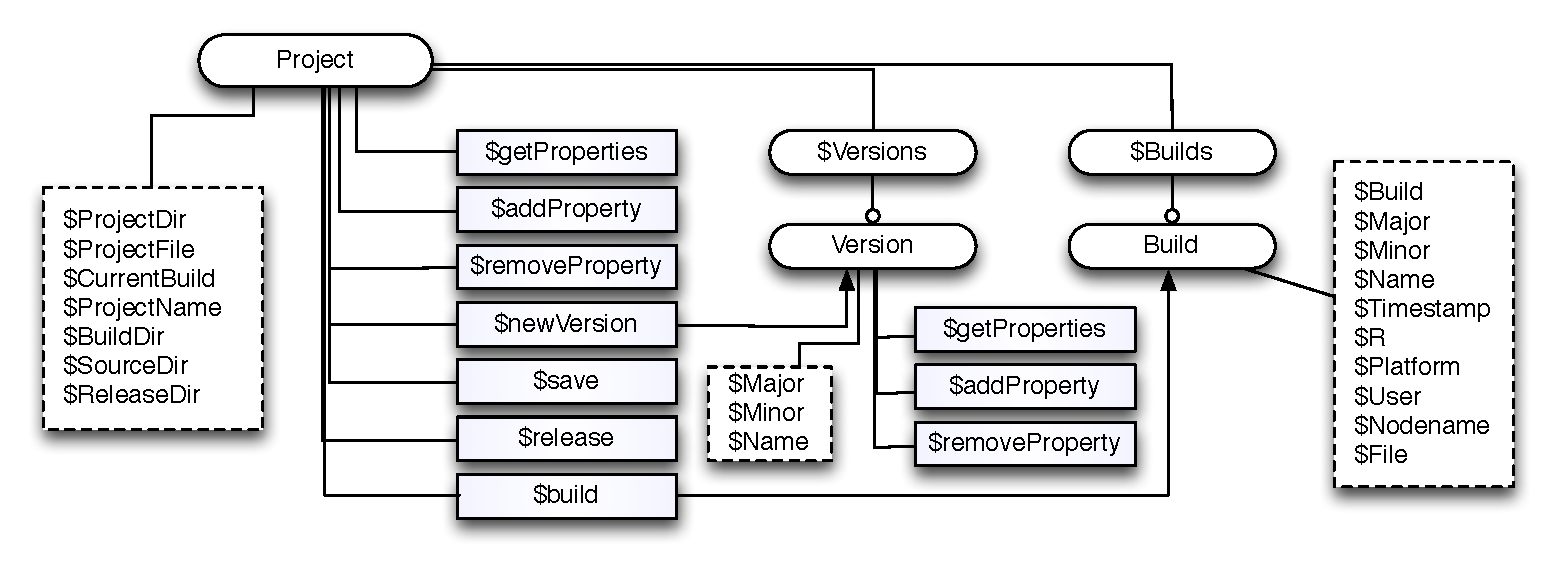
\includegraphics[width=\textwidth]{makeRClassDiagram.pdf}}
\caption{\label{figure:projectxml}\pkg{makeR} structure}
\end{figure*}

\section{Project framework}
There are three attributes to a particular document build, major (which can be numeric or character), minor, and build. Each major version is explicitly defined by the user. For example, if the goal of the project is to generate monthly reports then it would be appropriate to name each version using the month and year. Within each major version are minor versions. The minor version is always numeric and is incremented automatically upon each release. Lastly, build is a global numeric that is atomically incremented upon each document build. This index provides a unique identifier for each document that is created separate from the major and minor version identifiers.

From the perspective of the file system, the \pkg{makeR} package maintains a project file, \file{PROJECT.xml} (this will be discussed in further detail below), and three directories, \file{source}, \file{build}, and \file{release}. The \file{source} directory should contain an \file{.Rnw} file along with any support files. The entire contents of this directory, including any subdirectories, will be copied for each build. \pkg{makeR} will create a new subdirectory in \file{builds} for each unique major and minor combination. Lastly, the \file{release} directory will contain ``released" documents (i.e. final PDFs). The \code{releaseVersion} function will rename build files to include the major and minor versions.

Consider, for example, a new project that contains a file \file{Example.Rnw} in the \file{source} directory. Each call of the \code{buildVersion} function will copy all files from the \file{source} directory to the \file{builds/1.0} directory, the call \code{Stangle}, \code{Sweave}, and \code{texi2pdf} to create \file{builds/1.0/Example.pdf}. Calling \code{releaseVersion} will copy \file{bulids/1.0/Example.pdf} to \file{release/Example-1.0.pdf} and then increment the minor version so that subsequent calls to \code{buildVersion} will create the \file{builds/1.1} directory.

\section{Properties}
Properties are what differentiate one version from another and can be defined a the project level or version level. When \pkg{makeR} builds a document project level properties will be assigned before version level properties thereby giving version level properties priority over project level properties. The generic functions \code{addProperty} and \code{removeProperty}, whereby the first parameter is either objects of class type \code{Project} or \code{Version}, provide an interface for manipulating properties. 

\section{Package framework}
Figure \ref{figure:projectxml} depicts the internal representation of a \pkg{makeR} project. All interaction with a project will occur through the \code{Project} class object. By convention, all properties of classes begin with a capital letter and are represented in the boxes with dashed lined borders. Functions (or methods) begin with a lowercase letter and are represented in shaded boxes. Class objects and lists are represented by rounded squares. Project, Version, and Build are special classes for \pkg{makeR} whereas Versions and Builds are simply built in R lists. All manipulation of a project should be done through the appropriate functions. Although the attributes (i.e. elements of a list or class) are accessible given R's programming framework, doing so could result in unexpected results.

\section{Example}

The \href{http://www.r-bloggers.com}{R-Bloggers} site provides a wealth of information about R aggregated from many different R bloggers. Like many continuously changing data sources, we wish to periodically report on recent activity on the R-Bloggers site. The base source file, \file{rbloggers.Rnw}, is included in the package (in the \file{inst/doc/robloggers} directory) as well as being hosted on \href{https://github.com/jbryer/makeR/blob/master/inst/rbloggers/rbloggers.Rnw}{Github}. This example can also be run using \code{demo(makeR)}.

\subsection{Create new project}
\begin{example}
myProject = Project(name="RBloggers", 
  projectDir="~/rbloggers",
  properties=list(email=email, passwd=passwd))
\end{example}

\subsection{Create initial version}
\begin{example}
myProject$newVersion(myProject,
  name='2011-12', 
  properties=list(startDate='2011-12-01', 
  endDate='2011-12-31'))
\end{example}

\subsection{Building the document}
\begin{example}
myProject$build()
\end{example}

\subsection{Releasing the document}
\begin{example}
myProject$release()
\end{example}

\begin{figure}
\vspace*{.1in}
\framebox[\textwidth]{\raisebox{0in}{\rule{0in}{1in}}%
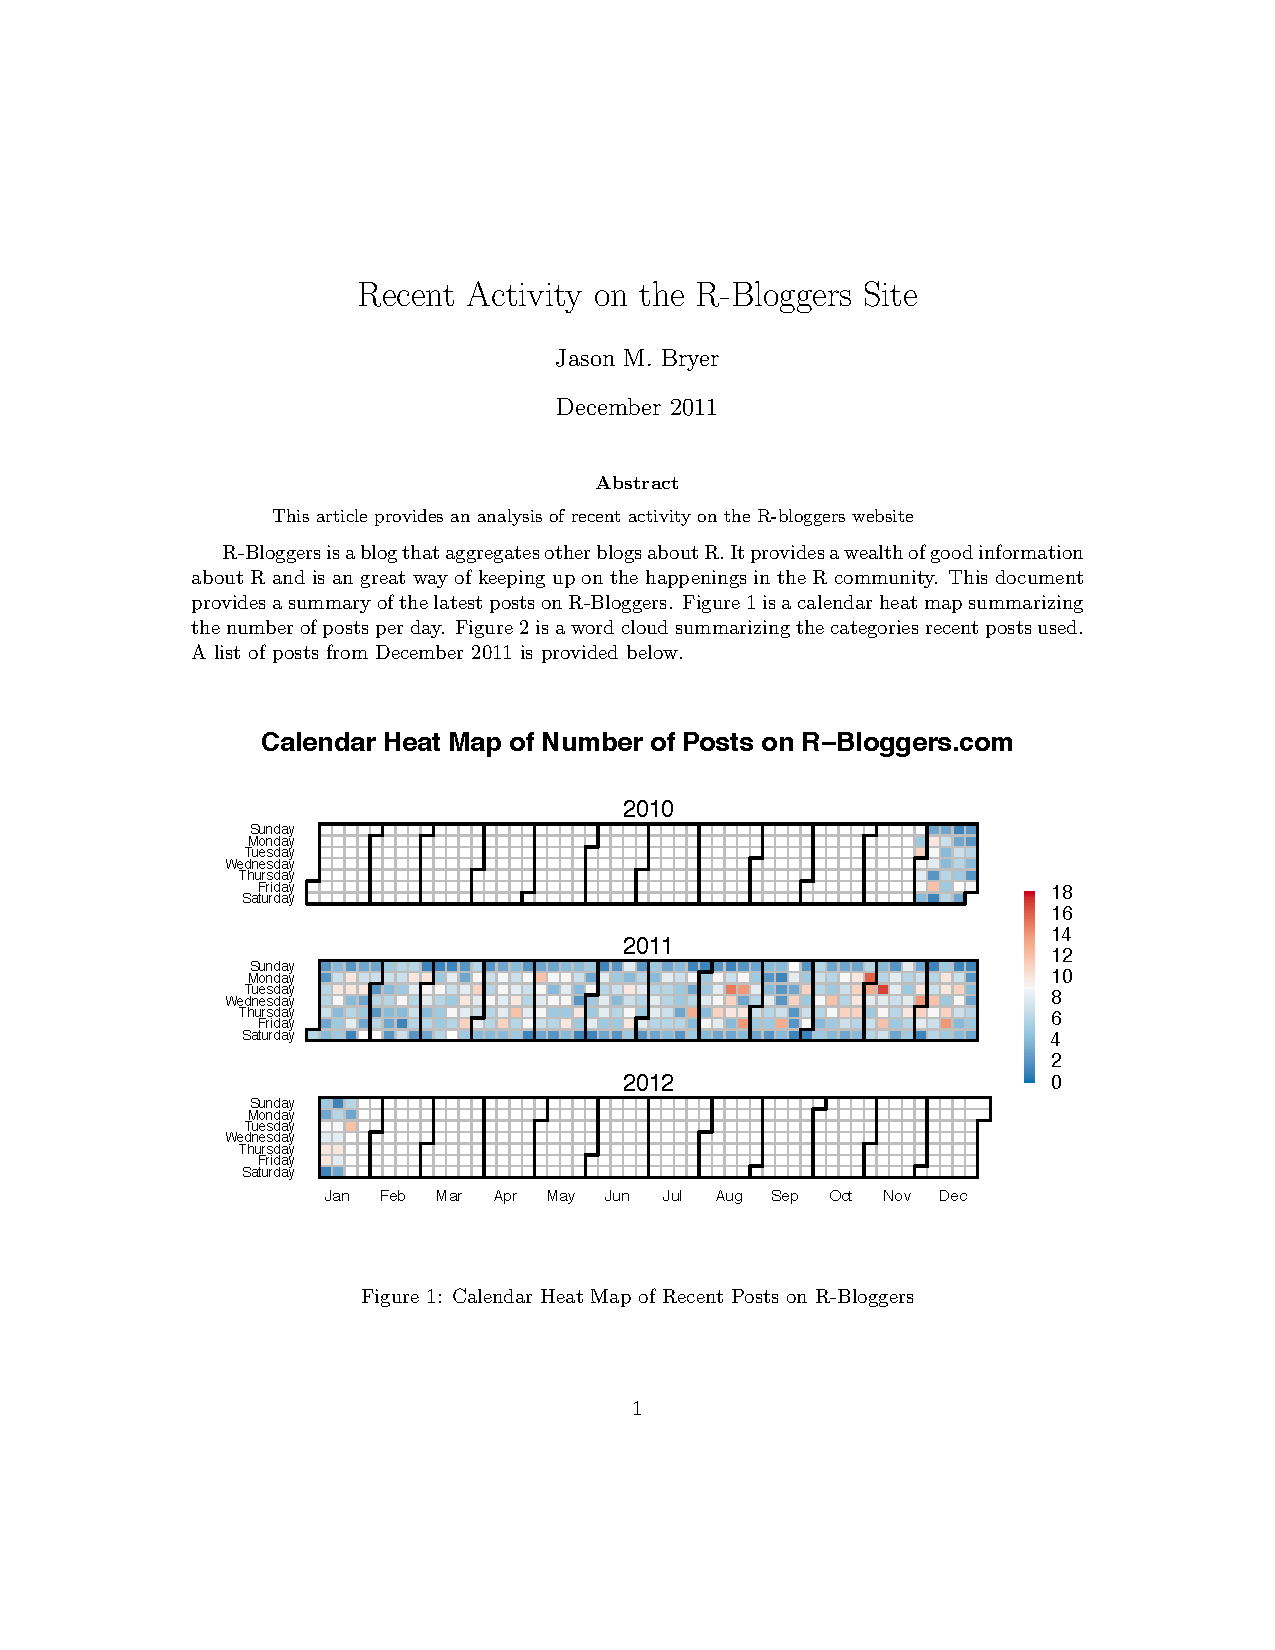
\includegraphics[width=\textwidth,trim=1cm 4cm 1cm 3cm,clip=true]{rbloggers.pdf}}%
\caption{\label{figure:rbloggers}%
Output from the R-Bloggers example.}%
\end{figure}


\section{The project file format}
\label{section:fileformat}

The \file{PROJECT.xml} file defines the properties, versions, and builds of a particular project. The file created and edited using the \pkg{XML} \citep{xml} package. Although the \pkg{makeR} package provides functions to manage projects, using XML allows for other R programmers to interact with the \pkg{makeR} project framework. Figure \ref{figure:projectxml} represents the contents of \file{PROJECT.xml} after running \code{demo(makeR)}.

\begin{figure*}
\vspace*{.1in}
%\framebox[\textwidth]{\hfill \raisebox{-.45in}{\rule{0in}{1in}}
\begin{example} 
<?xml version="1.0"?>
<project name="RBloggers" buildDir="build" releaseDir="release" sourceDir="source">
  <property name="email" value="GOOGLE READER USERNAME" type="character"/>
  <property name="passwd" value="GOOGLE READER PASSWORD" type="character"/>
  <versions>
    <version name="2011-12" major="1" minor="1">
      <property name="startDate" value="2011-12-01" type="character"/>
      <property name="endDate" value="2011-12-31" type="character"/>
    </version>
  </versions>
  <builds>
    <build major="1" minor="0" build="1" name="2011-12" timestamp="Wed Jan 18 12:29:51 2012" 
        R="R version 2.14.0 (2011-10-31)" platform="x86_64-apple-darwin9.8.0" 
        nodename="Jason-Bryers-MacBook-Air-2.local" 
        user="jbryer" file="rbloggers.pdf"/>
  </builds>
</project>
\end{example}
%}
\caption{\label{figure:projectxml}
\file{PROJECT.xml} for the R-Bloggers demo project.}
\end{figure*}

\section{Summary}


\section{Package development}
The latest stable version of \pkg{makeR} can be installed from your local CRAN server. Development versions are hosted on \href{http://github.com/jbryer/ProjectVersion}{Github}. The latest development version can be installed using the \pkg{devtools} \citep{devtools} package:

\begin{example}
install_github('makeR', 'jbryer')
\end{example}

\bibliography{Bibliography}

\address{Jason M. Bryer\\
  Excelsior College\\
  7 Columbia Circle\\
  Albany, NY 12203\\
  USA}\\
\email{jason@bryer.org}


%%%%%%%%%%%%%%%%%%%%%%%%%%%%%
\end{article}

\end{document}

